\chapter{Fundamental physics}
First, I will give a brief history of how the elementary particles were discovered.
Then I will describe their subsummation in the Standard Model.

\section{History}

The year in which particle physics was conceived is a fungible number,
but a strong case could be made for 1897, 
when Sir Joseph John Thomson discovered the electron \cite{Thomson1897}.
The following decades brought Ernest Rutherford's atomic nuclei in 1911 \cite{Rutherford1911}, 
Niels Bohr's atomic model in 1913 \cite{Bohr1913}, 
and then James Chadwick's neutron in 1932 \cite{Chadwick1932}.

After the electron, the next elementary particle discovered was the photon.
The evidence was provided by: 
Max Planck's study of quantized blackbody radiation in 1900 \cite{Planck1901};
Albert Einstein's controversial explanation of the photoelectric effect in 1905 \cite{Einstein1905};
and Arthur Holly Compton's scattering experiment in 1923 \cite{Compton1923}.

In 1935, Yukawa Hideki proposed a light, yet massive meson to mediate the nucleon interaction \cite{Yukawa1935}.
By 1937, multiple efforts searching for Yukawa's meson in the cosmic rays, instead found an impostor.
This was the next elementary particle, the muon ($\mu^-$): a second-generation charged lepton \cite{Stevenson1937} \cite{Anderson1937}.

The so-called Yukawa meson really did exist, although it was not discovered until 1947 at the University of Bristol \cite{Lattes1947}.
Today we call it the charged pion ($\pi^\pm$), and it is a composite subatomic particle, 
not an elementary one. But in hindsight, 
this was our initial foray into the strong nuclear force,
since we continue to describe the force between proximate nucleons
via the exchange of one or more such light, virtual mesons.

After the discovery of the neutron, Enrico Fermi and Wolfgang Pauli's work in the early 1930s 
led to the prediction of the neutrino, another elementary particle \cite{Fermi1934}. 
It was not discovered until 1956 by Clyde Cowan and Frederick Reines using inverse beta decay \cite{Cowan1956}.
This was our first conception of the weak nuclear force. 
The second and third generation neutrinos came later. 
Lederman, Schwartz, and Steinberger observed the second-generation muon neutrino 
($\nu_\mu$) in 1962 \cite{Lederman1962}.

The third-generation charged lepton, the tau ($\tau$), was discovered at the Stanford Linear Accelerator Center in 1975 \cite{Perl1975}.
The DONUT experiment observed its partner, the tau neutrino ($\nu_\tau$), in 2000 \cite{Donut2001}.

The constituents of mesons and atomic matter were found to be the quarks, 
Most of the quarks can be bound together for a time by gluons. 
Quarks, or aces, were originally conceived of by Murray Gell-Mann \cite{GellMann:1964nj} and George Zweig \cite{Zweig:570209}.
Briefly, the order of their observation is as follows: 
the up, down, and strange quarks in 1968 \cite{PhysRevLett.23.930} \cite{PhysRevLett.23.935};
the charm quark 1974 \cite{Ting1974} \cite{Richter1974};
the bottom quark in 1977 \cite{Lederman1977};
the gluon in 1978; \cite{Stella2011}
and the top quark in 1995 \cite{CDFTop1995} \cite{D0Top1995}.

The unified electroweak theory was validated when the $\W^\pm$ and $\Z$ bosons 
were discovered in 1983 by the UA1 and UA2 experiments 
\cite{Arnison:1983mk} \cite{Arnison:1983rp} \cite{Bagnaia:1983zx} \cite{Banner:1983jy}. 
Finally, the last missing component of the Standard Model, the Higgs boson, was discovered in 2012 by the CMS and ATLAS collaborations \cite{Chatrchyan:2012xdj} \cite{Aad:2012tfa}.

The Standard Model of particle physics was built up over a century of arduous and incremental observations. Thus, the remainder of this work is written standing on the shoulders of giants.

\section{Standard Model}
%\setlength{\mathindent}{12pt}
Now I will present the individual interactions and their unification in the theory.
Beyond the scope of this work are discussions of gravitation, general relativity, and
previous theories of yore.

The internal symmetries of the Standard Model are represented by the unitary product group 
$\mathrm{SU}(3) \times \mathrm{SU}(2) \times \mathrm{U}(1)$.

The Lagrangian density of the Standard Model can be deconstructed as
\begin{equation}
\mathcal{L}_\mathrm{SM} = \mathcal{L}_\mathrm{EW} + \mathcal{L}_\mathrm{QCD}
\end{equation}
I will describe each of the components below.

\subsection{Electromagnetic force}
\label{qed}
The quantum field theory for electromagnetism is quantum electrodynamics or QED for short,
with internal symmetry represented by the group $\mathrm{U}(1)$. 
QED was the first quantum field theory to incorporate special relativity. 
It describes the interactions between charged particles, the force being carried by the photon.
The Lagrangian density for a fermion field interacting with the electromagnetic field is

\begin{equation}
\mathcal{L}_\mathrm{QED} = \bar{\psi}\left( i\gamma^\mu D_\mu - m \right) \psi - \frac{1}{4} F_{\mu\nu} F^{\mu\nu}
\end{equation}

\begin{itemize}
  \setlength\itemsep{0em}
  \item The indices $\mu,\nu$ represent spacetime.
  \item $e$ is the coupling constant, also known as the elementary charge of the electron.
  \item $\gamma^\mu$ are the Dirac matrices which act on Dirac spinors to produce four-vectors.
  \item $\psi$ is a Dirac bi-spinor representing the field for a charged spin-1/2 particle and antiparticle e.g. an electron and positron at spacetime point $x$.
  \item $m$ is the mass of that particle.
  \item $\bar{\psi}$ is the Dirac adjoint of $\psi$, defined as $\psi^\dagger \gamma^0$.
  \item $D_\mu$ is the gauge covariant derivative $\partial_\mu + ieA_\mu + ieB_\mu$.
  \item $A_\mu$ is the electromagnetic four-potential from the particle itself.
  \item $B_\mu$ is the external EM four-potential.
  \item $F_{\mu\nu}$ is the electromagnetic field tensor $\partial_\mu A_\nu - \partial_\nu A_\mu$.
\end{itemize}

In QED there is only the fermion-fermion-photon vertex. 
This quantum field theory offered uncanny accuracy for observables such as
the energy levels of the hydrogen atom and the anomalous magnetic moment of the electron.
It has been subsumed into the electroweak theory, which will be described next.

\subsection{Electroweak unification}
\label{electroweak}
The weak interaction describes the interactions between fermions.
The conserved quantum number is the weak isospin ($T^3$).
The classic example is beta decay, where a down quark ($T^3={-}1/2$) changes into an up quark ($T^3=+1/2$),
producing an additional electron and electron antineutrino (both $T^3={-}1/2$). 
In such a process, the weak isospin, electron number, and charge are all conserved.
A historical discussion of the weak interaction alone is omitted.

The electromagnetic and weak nuclear forces are unified in the theory of electroweak (EW) interactions,
wrought by Sheldon Glashow, Steven Weinberg, and Abdus Salam (GWS).
Above unification energy circa 250 \GeV, or temperature $10^{15}$ Kelvins, these forces are merged into a combined force.
EW is a Yang-Mills theory based on the gauge group $\mathrm{SU}(2) \times \mathrm{U}(1)$.
The $\mathrm{SU}(2)$ group represents the three gauge bosons of weak isospin, 
$\mathrm{A}_1$, $\mathrm{A}_2$, and $\mathrm{A}_3$.
The $\mathrm{U}(1)$ group represents the gauge boson $\mathrm{B}$ of weak hypercharge.
All of these gauge bosons are massless. 
The coupling constants are $g$ for $\mathrm{SU}(2)$ and $g'$ for $\mathrm{U}(1)$.

The left-handed fermion fields transform as doublets under SU(2).
The lepton doublets are $L_i = \begin{pmatrix}\nu_i \\ \ell_i^{-} \end{pmatrix}$ where $\nu_i$ are the three neutrinos and $\ell_i^{-}$ are the three charged leptons.
The quark doublets are $Q_i = \begin{pmatrix} u_i \\ V_{ij} d_j \end{pmatrix}$, 
where $u_i$ are the three up-type quarks, $d_j$ are the three down-type quarks,
and $V_{ij}$ is the Cabibbo-Kobayashi-Maskawa (CKM) matrix describing the weak mixing among the quark generations.

The Lagrangian density for the pure, unadulterated electroweak interaction is
\begin{equation}
\begin{split}
\label{eq:EWpreSSB}
\mathcal{L}_\mathrm{EW} & = \mathcal{L}_\mathrm{Gauge} + \mathcal{L}_\mathrm{Fermion} + \mathcal{L}_\mathrm{\phi} + \mathcal{L}_\mathrm{Yukawa} \:\:\mathrm{where} \\
\mathcal{L}_\mathrm{Gauge}   & = -\frac{1}{4}A^{\mu\nu}_a A^a_{\mu\nu} - \frac{1}{4} B^{\mu\nu} B_{\mu\nu} \\
\mathcal{L}_\mathrm{Fermion} & = \sum_{f \in \{Q,u,d,L,i\}} \bar{f}_i i \gamma_\mu D^\mu f_i \\ 
\mathcal{L}_\mathrm{\phi}   & = |D_\mu \phi|^2 - \lambda \left( |\phi|^2 - \frac{1}{2} v^2 \right)^2 \\
%\mathcal{L}_\mathrm{Yukawa}  & = -y_u^{ij} \epsilon^{ab} \phi_b^\dagger \bar{Q}_{ia} u^c_j - y_d^{ij} \phi \bar{Q}_i d^c_j - y_e^{ij} \phi \bar{L}_i e^c_j + \mathrm{h.c.}
\mathcal{L}_\mathrm{Yukawa}  & = \sum_f -G_f (\bar{f}_\mathrm{L.H.} \phi f_\mathrm{R.H.} + \bar{f}_\mathrm{R.H.} \phi^\dagger f_\mathrm{L.H.} )
\end{split}
\end{equation}
Breaking it down piece by piece, 
\begin{itemize}
  \setlength\itemsep{0em}
  \item $\mathcal{L}_\mathrm{Gauge}$ is the interaction among the gauge fields, described by the field strength tensors $A_{1,2,3}^{\mu\nu}$ and $B^{\mu\nu}$ for the weak isospin and weak hypercharge gauge fields.
  \item $\mathcal{L}_\mathrm{Fermion}$ is the interaction of the gauge bosons and the fermions. $f$ represents the left-handed doublet quark fields, the right-handed singlet up-type quark fields, the right-handed singlet down-type quark fields, the left-handed doublet lepton fields, and the right-handed singlet lepton fields. 
  \item $D_\mu$ is the electroweak gauge covariant derivative, defined as 
    $\partial_\mu - i\frac{g}{2} \hat{T}^j A^{j}_{\mu} - i \frac{g'}{2} Y B_\mu $ where $\hat{T}^{j=1,2,3}$ are the weak isospin operators and $\hat{Y}$ is the weak hypercharge operator. 
  \item $\mathcal{L}_\mathrm{\phi}$ is the scalar field's interaction with itself and the gauge bosons.
  \item $\mathcal{L}_\mathrm{Yukawa}$ is the Yukawa interaction of the scalar field with the fermions $f$, where $f_\mathrm{L.H.}, f_\mathrm{R.H.}$ are the left-handed and right-handed fermion fields.
\end{itemize}

\subsection{Spontaneous symmetry breaking}
\label{higgs}

Motivated by the necessity to generate the masses, a complex scalar doublet field is added for this purpose:
\begin{equation}
\phi \equiv \begin{pmatrix} \phi^+ \\ \phi^0 \end{pmatrix}, \:\:\mathrm{where~} \phi^+, \phi^0 \:\mathrm{are~complex~numbers}
\end{equation}
This $\phi$ field lives in a potential given by 
\begin{equation}
V(\phi) = \mu^2 \phi^\dagger \phi + \lambda (\phi^\dagger \phi)^2 \label{eq:higgsV}
\end{equation}
$\lambda$ must be positive in order for the potential $V$ to have a minimum.
For negative values of the constant $\mu$, $V$ could be visualized as a sombrero or similar hat with a rounded brim.
Since the lowest point is somewhere in the brim, 
the $\phi$ doublet develops a vacuum expectation value $v/\sqrt{2}$.
This breaks the SU(2) symmetry, but a new U(1) symmetry is maintained.
The value of $v$ is experimentally found to be around 246 \GeV,
providing a basis for the earlier statement about the unification energy.

Undertaking a unitary gauge transformation in SU(2), $\phi^+$ vanishes and $\phi^0$ remains as a physical scalar field.
Expanding this scalar field around the minimum of the potential in Equation~\ref{eq:higgsV}, $\phi^0 \rightarrow \frac{v+H(x)}{\sqrt{2}}$,
where $H(x)$ is a scalar at spacetime position $x$ with expected value 0.

Symmetry breaking alters the terms $\mathcal{L}_\mathrm{\phi}$ and $\mathcal{L}_\mathrm{Yukawa}$ in Equation~\ref{eq:EWpreSSB}, leaving the others unchanged. In a Lagrangian density, the kinetic and potential terms for such a scalar field $\phi$ are
\begin{equation}
\mathcal{L}_\phi = (D_\mu\phi)^\dagger(D^\mu\phi) - V(\phi) \label{eq:Lphi}
\end{equation}
Let us expand Equation~\ref{eq:Lphi} for the $\phi$-field using the previously defined $D_\mu$:
\begin{equation}
\begin{split}
%\mathcal{L}_\mathrm{Yukawa}  & = \sum_f -G_f \bar{f} f (v+H) \\
\mathcal{L}_\mathrm{\phi} & = \frac{1}{2} (\partial^\mu H) (\partial_\mu H) - \lambda\left[ v^2H^2 + vH^3 + \frac{1}{4}H^4\right] \\
& + \frac{1}{8} \left| g \hat{T}^1 A^1_\mu + g \hat{T}^2 A^2_\mu + g \hat{T}^3 A^3_\mu + g' Y B_\mu \right|^2 (v+H)^2
\end{split}
\end{equation}
Noting that $(\hat{T}^1 \pm i \hat{T}^2)/2 \equiv \hat{T}^\pm$ are the raising and lowering operators 
for the third component of weak isospin in the SU(2) symmetry,
and the charge operator $\hat{Q} = \hat{T}^3 - \hat{Y}$,
the last term in $\mathcal{L}_\mathrm{\phi}$ simplifies:
\begin{equation}
\mathcal{L}_\mathrm{\phi} = ... + \frac{1}{8}\left[ g^2(A^1_\mu)^2 + g^2(A^2_\mu)^2  + \left( gA^3_\mu + g' B_\mu \right)^2 \right] (v+H)^2
\end{equation}
If we define a weak angle $\theta_W = \mathrm{arctan}\frac{g'}{g}$, 
we view $gA^3_\mu + g' B_\mu$ as the $A^3$ and B bosons being rotated into two other bosons. 
These will be the massive Z boson and the massless $\gamma$ boson, also known as the photon \cite{Weinberg1967}.
Meanwhile, we can view the $A^1$ and $A^2$ bosons combining to give the charged $W^\pm$ bosons:
\begin{equation}
W^\pm = \frac{A^1 \mp iA^2}{\sqrt{2}} \label{eq:WpmA12}
\end{equation}
For completeness, let us rewrite the electroweak gauge covariant derivative in terms of the physical bosons.
The Z boson is represented by the gauge field $Z_\mu$ and the photon is represented by the gauge field $A_\mu$ without a superscript.
\begin{equation}
\label{eq:covariant_derivative}
D_\mu^\mathrm{EW} = \partial_\mu - \frac{ig}{\sqrt{2}} (W_\mu^+ \hat{T}^+ + W_\mu^- \hat{T}^-) - \frac{ig}{\mathrm{cos}\:\theta_W} Z_\mu( \hat{T}^3 - \mathrm{sin}^2 \: \theta_W \: \hat{Q}) - ie A_\mu \hat{Q}
\end{equation}
We can now rewrite $\mathcal{L}_\mathrm{\phi}$ from before, in terms of the physical W and Z bosons:
\begin{equation}
\label{eq:LhiggsWZ}
\begin{split}
\mathcal{L}_\mathrm{\phi} & = \frac{1}{2} (\partial^\mu H) (\partial_\mu H) - \lambda\left[ v^2H^2 + vH^3 + \frac{1}{4}H^4\right] \\
& + \left[ \frac{g^2}{4} W^+_\mu W^{{-}\mu}  + \frac{g^2}{8\:\mathrm{cos}^2\:\theta_W} Z_\mu Z^\mu \right](v+H)^2   \\
\end{split}
\end{equation}
From this expression, we can extract expressions for the W and Z bosons' masses at leading-order:
\begin{equation}
\label{eq:WZmass}
m_W = \frac{v g}{2},\:\:\:\:m_Z = \frac{vg}{2\:\mathrm{cos}\:\theta_W}
\end{equation}
Lastly, why don't we reframe Equation~\ref{eq:EWpreSSB} in terms of the physical gauge bosons.
The photon, Z, and W field strength tensors $A_{\mu\nu}$, $A_{\mu\nu}$, $A_{\mu\nu}$, $A_{\mu\nu}$ are provided as
\begin{equation}
\begin{split}
blah
\end{split}
\end{equation}
Finally, we can write down the full EW Lagrangian density after symmetry breaking. 
As before, $\mathcal{L}_\mathrm{EW} = \mathcal{L}_\mathrm{Gauge} + \mathcal{L}_\mathrm{Fermion} + \mathcal{L}_\mathrm{\phi} + \mathcal{L}_\mathrm{Yukawa}$. 

The $\mathcal{L}_\mathrm{Gauge}$ term contains the gauge field tensor dynamic terms, the triple-gauge couplings, and the quartic-gauge couplings:
\begin{equation} 
\begin{split}
\label{eq:L_Gauge}
\mathcal{L}_\mathrm{Gauge} & = -\frac{1}{4} \termLB A^{\mu\nu} A_{\mu\nu} - 2  W^+_{\mu\nu} W^{{-}\mu\nu} - Z_{\mu\nu} Z^{\mu\nu} \termRB  \\ 
 & - ig \termLB (W^+_{\mu\nu} W^{{-}\mu} - W^{+\mu} W^{{-}}_{\mu\nu})(A^\nu\mathrm{sin}\:\theta_W - Z^\nu \mathrm{cos}\:\theta_W)  \\
 & \qquad\qquad\qquad\qquad\qquad\qquad + W^{{-}}_{\nu} W^+_{\mu} (A^{\mu\nu} \mathrm{sin}\:\theta_W - Z^{\mu\nu} \mathrm{cos} \theta_W ) \termRB  \\
 & + \frac{g^2}{4} \termLB {-}\big( 2 W^+_\mu W^{{-}\mu} + (A_\mu \mathrm{sin}\:\theta_W - Z_\mu \mathrm{cos}\:\theta_W)^2 \big)^2 \\
 & \:\: + \big( W_\mu^+ W_\nu^{{-}} + W_\nu^+ W_\mu^{{-}} + (A_\mu \mathrm{sin}\:\theta_W - Z_\mu \mathrm{cos}\:\theta_W)(A_\nu\mathrm{sin}\:\theta_W - Z_\nu \mathrm{cos}\:\theta_W)\big)^2 \termRB
\end{split}
\end{equation}
The allowed gauge self-coupling vertices are pictured in Figures~\ref{fig:3GC} and~\ref{fig:4GC}.

The $\mathcal{L}_\mathrm{Fermion}$ term contains the interaction between the gauge bosons and the fermions, in the neutral current and the charged current:
\begin{equation}
\begin{split}
\label{eq:L_Fermion}
\mathcal{L}_\mathrm{Fermion} & = \termLB \frac{g}{\mathrm{cos}\:\theta_W} \big(J_\mu^\mathrm{3} - \mathrm{sin}^2\:\theta_W J_\mu^\mathrm{EM} \big) Z^\mu + eJ_\mu^\mathrm{EM} A^\mu \termRB \\
& - \frac{g}{\sqrt{2}} \termLB \big( \bar{u}_i \gamma^\mu \frac{1-\gamma^5}{2} V_{ij} d_j + \bar{\nu}_i \gamma^\mu \frac{1-\gamma^5}{2} e_i \big) W_\mu^+ + \mathrm{h.c.} \termRB
\end{split}
\end{equation}

The electromagnetic current is defined as $J^\mathrm{EM}_\mu \equiv \sum_f q_f \bar{f} \gamma_\mu f$ , with the bilinear covariant $\gamma_\mu$ representing the vector spin-1 coupling.
The weak neutral current is defined as $J^\mathrm{3}_\mu \equiv \sum_f T^3_f \bar{f} \gamma_\mu \frac{1-\gamma^5}{2} f$,
with the bilinear covariant representing the infamous ``vector minus axial'' spin-1 coupling.
The matrix $V_{ij}$ is the CKM matrix.

%This model is renormalizable

%\mathcal{L}_\mathrm{Fermion} & = \termLB \big( e A^\mu \sum_f q_f \bar{f} \gamma_\mu f \big) + \big( \frac{gZ^\mu}{\mathrm{cos}\:\theta_W}( \big)\termRB
%\mathcal{L}_\mathrm{Fermion} & = \sum_{f} \bar{f} i \gamma^\mu \partial_\mu - m_f) f \nonumber \\ 
%\mathcal{L}_\mathrm{\phi}    & = |D_\mu \phi|^2 - \lambda \left( |\phi|^2 - \frac{1}{2} v^2 \right)^2 \nonumber \\
%\mathcal{L}_\mathrm{Yukawa}  & = {-} \sum_f \frac{gm_f}{2m_W} \bar{f} f H \nonumber
%\end{align}
\begin{figure}[!hbt] % 3GC
 \centering
 \begin{tikzpicture} % WWZ
  \begin{feynman}
   \vertex (a2) {\(\boldsymbol{\W^\pm}\)};
   \vertex [right= 1.5cm of a2] (b1);
   \vertex [right= 1.1cm of b1] (c1);
   \vertex [above= 0.9cm of c1] (c2) {\(\boldsymbol{\Z}\)};
   \vertex [below= 0.9cm of c1] (c3) {\(\boldsymbol{\W^\pm}\)};
   
   \diagram* {
    (a2) -- [boson, very thick] (b1),
    (b1) -- [boson, very thick] (c2),
    (b1) -- [boson, very thick] (c3),
   };
  \end{feynman}
 \end{tikzpicture} \hspace{0.5cm}
 \begin{tikzpicture} % WWy
  \begin{feynman}
   \vertex (a2) {\(\boldsymbol{\W^\pm}\)};
   \vertex [right= 1.5cm of a2] (b1);
   \vertex [right= 1.1cm of b1] (c1);
   \vertex [above= 0.9cm of c1] (c2) {\(\boldsymbol{\gamma}\)};
   \vertex [below= 0.9cm of c1] (c3) {\(\boldsymbol{\W^\pm}\)};
   
   \diagram* {
    (a2) -- [boson, very thick] (b1),
    (b1) -- [boson, very thick] (c2),
    (b1) -- [boson, very thick] (c3),
   };
  \end{feynman}
 \end{tikzpicture} 
 \caption{Triple gauge boson vertices in the electroweak theory.} \label{fig:3GC}
\end{figure}

\begin{figure}[!hbt] % 4GC
 \centering
 \begin{tikzpicture} % WWWW
  \begin{feynman}
   \vertex (a1);
   \vertex [above= 0.8cm of a1] (a2) {\(\boldsymbol{\W}\)};
   \vertex [below= 0.8cm of a1] (a3) {\(\boldsymbol{\W}\)};
   \vertex [right= 1.2cm of a1] (b1);
   \vertex [right= 1.2cm of b1] (c1);
   \vertex [above= 0.8cm of c1] (c2) {\(\boldsymbol{\W}\)};
   \vertex [below= 0.8cm of c1] (c3) {\(\boldsymbol{\W}\)};
   
   \diagram* {
    (a2) -- [boson, very thick] (b1),
    (a3) -- [boson, very thick] (b1),
    (b1) -- [boson, very thick] (c2),
    (b1) -- [boson, very thick] (c3),
   };
  \end{feynman}
 \end{tikzpicture} \hspace{0.5cm}
 \begin{tikzpicture} % WWyy
  \begin{feynman}
   \vertex (a1);
   \vertex [above= 0.8cm of a1] (a2) {\(\boldsymbol{\W}\)};
   \vertex [below= 0.8cm of a1] (a3) {\(\boldsymbol{\W}\)};
   \vertex [right= 1.2cm of a1] (b1);
   \vertex [right= 1.2cm of b1] (c1);
   \vertex [above= 0.8cm of c1] (c2) {\(\boldsymbol{\gamma}\)};
   \vertex [below= 0.8cm of c1] (c3) {\(\boldsymbol{\gamma}\)};
   
   \diagram* {
    (a2) -- [boson, very thick] (b1),
    (a3) -- [boson, very thick] (b1),
    (b1) -- [boson, very thick] (c2),
    (b1) -- [boson, very thick] (c3),
   };
  \end{feynman}
 \end{tikzpicture} \hspace{0.5cm}
 \begin{tikzpicture} % WWyZ
  \begin{feynman}
   \vertex (a1);
   \vertex [above= 0.8cm of a1] (a2) {\(\boldsymbol{\W}\)};
   \vertex [below= 0.8cm of a1] (a3) {\(\boldsymbol{\W}\)};
   \vertex [right= 1.2cm of a1] (b1);
   \vertex [right= 1.2cm of b1] (c1);
   \vertex [above= 0.8cm of c1] (c2) {\(\boldsymbol{\gamma}\)};
   \vertex [below= 0.8cm of c1] (c3) {\(\boldsymbol{\Z}\)};
   
   \diagram* {
    (a2) -- [boson, very thick] (b1),
    (a3) -- [boson, very thick] (b1),
    (b1) -- [boson, very thick] (c2),
    (b1) -- [boson, very thick] (c3),
   };
  \end{feynman}
 \end{tikzpicture} \hspace{0.5cm}
 \begin{tikzpicture} % WWZZ
  \begin{feynman}
   \vertex (a1);
   \vertex [above= 0.8cm of a1] (a2) {\(\boldsymbol{\W}\)};
   \vertex [below= 0.8cm of a1] (a3) {\(\boldsymbol{\W}\)};
   \vertex [right= 1.2cm of a1] (b1);
   \vertex [right= 1.2cm of b1] (c1);
   \vertex [above= 0.8cm of c1] (c2) {\(\boldsymbol{\Z}\)};
   \vertex [below= 0.8cm of c1] (c3) {\(\boldsymbol{\Z}\)};
   
   \diagram* {
    (a2) -- [boson, very thick] (b1),
    (a3) -- [boson, very thick] (b1),
    (b1) -- [boson, very thick] (c2),
    (b1) -- [boson, very thick] (c3),
   };
  \end{feynman}
 \end{tikzpicture}
 \caption{Non-Abelian quartic gauge couplings in the electroweak theory.} \label{fig:4GC}
\end{figure}

\subsection{The Higgs boson}

Let us look at the second term of Equation~\ref{eq:LhiggsWZ}.
The portion $-\lambda v^2 H^2 $ suggests to us we can identify the quantum of the $H$-field as a physical boson with mass $m_H = \sqrt{2v^2\lambda}$.
Finally, I will drop the act and call a spade a spade:
This quantum is none other than the Higgs boson, and we can call the field the Higgs field.

The $\mathcal{L}_\mathrm{\phi}$ term from the electroweak Lagrangian density can be expanded to find the Higgs couplings to itself and the other gauge bosons, in particular to the Z boson which is relevant to this work:

\begin{equation}
\begin{split}
\label{eq:L_phi}
\mathcal{L}_\mathrm{\phi} & = \termLB \frac{1}{2} (\partial^\mu H) (\partial_\mu H) - \frac{1}{2}m_H^2 H^2 \termRB - \termLB \frac{gm_H^2}{4m_W} H^3 + \frac{g^2m_H^2}{32m_W^2}H^4 \termRB \\
& + \termLB \left( W_\mu^+ W^{{-}\mu} + \frac{1}{2\mathrm{cos}^2\:\theta_W} Z_\mu Z^\mu \right) \left( gm_WH+\frac{g^2}{4}H^2 \right) \termRB
\end{split}
\end{equation}

Meanwhile, the $\mathcal{L}_\mathrm{Yukawa}$ term from the Lagrangian density becomes
\begin{equation}
\label{L_Yukawa}
\mathcal{L}_\mathrm{Yukawa} = {-} \sum_f \frac{gm_f}{2m_W} \bar{f}fH
\end{equation}
It provides for the Higgs boson to interact with and decay into fermions,
more likely for massive fermions.
The fermion mass $m_f$ truly arises from the coupling to the Higgs field, and not vice versa.

\begin{figure}[!hbt] % Higgs couplings
 \centering
\begin{tikzpicture} % VVH
  \begin{feynman}
   \vertex (a2) {\(\boldsymbol{\mathrm{V}}\)};
   \vertex [right= 1.3cm of a2] (b1);
   \vertex [right= 1.1cm of b1] (c1);
   \vertex [above= 0.9cm of c1] (c2) {\(\boldsymbol{\Hi}\)};
   \vertex [below= 0.9cm of c1] (c3) {\(\boldsymbol{\mathrm{V}}\)};
   
   \diagram* {
    (a2) -- [boson, very thick] (b1),
    (b1) -- [scalar, very thick] (c2),
    (b1) -- [boson, very thick] (c3),
   };
  \end{feynman}
 \end{tikzpicture} \hspace{0.5cm}
 \begin{tikzpicture} % Hff
  \begin{feynman}
   \vertex (a2) {\(\boldsymbol{f}\)};
   \vertex [right= 1.3cm of a2] (b1);
   \vertex [right= 1.1cm of b1] (c1);
   \vertex [above= 0.9cm of c1] (c2) {\(\boldsymbol{\Hi}\)};
   \vertex [below= 0.9cm of c1] (c3) {\(\boldsymbol{f}\)};
   
   \diagram* {
    (a2) -- [fermion, very thick] (b1),
    (b1) -- [scalar, very thick] (c2),
    (b1) -- [fermion, very thick] (c3),
   };
  \end{feynman}
 \end{tikzpicture} \hspace{0.5cm}
 \begin{tikzpicture} % HHH
  \begin{feynman}
   \vertex (a2) {\(\boldsymbol{\Hi}\)};
   \vertex [right= 1.3cm of a2] (b1);
   \vertex [right= 1.1cm of b1] (c1);
   \vertex [above= 0.9cm of c1] (c2) {\(\boldsymbol{\Hi}\)};
   \vertex [below= 0.9cm of c1] (c3) {\(\boldsymbol{\Hi}\)};
   
   \diagram* {
    (a2) -- [scalar, very thick] (b1),
    (b1) -- [scalar, very thick] (c2),
    (b1) -- [scalar, very thick] (c3),
   };
  \end{feynman}
 \end{tikzpicture} \hspace{0.5cm}
 \begin{tikzpicture} % HHHH
  \begin{feynman}
   \vertex (a1);
   \vertex [above= 0.8cm of a1] (a2) {\(\boldsymbol{\Hi}\)};
   \vertex [below= 0.8cm of a1] (a3) {\(\boldsymbol{\Hi}\)};
   \vertex [right= 1.2cm of a1] (b1);
   \vertex [right= 1.2cm of b1] (c1);
   \vertex [above= 0.8cm of c1] (c2) {\(\boldsymbol{\Hi}\)};
   \vertex [below= 0.8cm of c1] (c3) {\(\boldsymbol{\Hi}\)};
   
   \diagram* {
    (a2) -- [scalar, very thick] (b1),
    (a3) -- [scalar, very thick] (b1),
    (b1) -- [scalar, very thick] (c2),
    (b1) -- [scalar, very thick] (c3),
   };
  \end{feynman}
 \end{tikzpicture}
 \caption{Higgs boson couplings. V is a $\W^\pm$ or $\Z$ boson. $f$ are fermions.}
\end{figure}


\subsection{Strong nuclear force}

The strong nuclear force arises from the theory of the interactions of the quarks and the gluon, called quantum chromodynamics (QCD).
It is a non-Abelian gauge theory whose internal symmetry is represented by the group $\mathrm{SU}(3)$.

Quarks and gluons carry color charge, of which there are three kinds: red, green, and blue.
Negative color charge, carried by the antiquarks and the gluons, is usually represented by the prefix \textit{anti-}, e.g. anti-red.
In transmitting the strong force as its carrier, the gluon carries a positive color charge and a negative color charge.
A gluon could carry red and anti-blue color charge, for example.
There are eight such possible combinations, each of which is a different kind of gluon.
These eight gluons correspond to the eight generators of the $\mathrm{SU}(3)$ group.

Quarks are fermions, having intrinsic spin of 1/2. There are six quarks.
Each quark has a bare mass and an electric charge.
In bound states such as the proton, the quarks appear to weigh more.
This constituent quark mass is heavier because of the field of virtual quarks and gluons around the bare quarks.

\begin{table}[ht]
  \caption{The quarks. When significant, bare masses quote statistical followed by systematic uncertainty. \label{tab:quarks}}
  \begin{center} {\scriptsize
  \begin{tabular}{|p{1.5cm}|c|c|c|c|c|}
  \hline
  \bf{Quark} & \bf{Symbol} & \bf{Charge} & \bf{Isospin} & \bf{Bare mass} $\mathbf{[\MeV\:c^{-2}]}$ & \bf{Constituent mass} $\mathbf{[\MeV\:c^{-2}]}$ \\
  \hline
  Up         & $u$         & {+2/3}      & +1/2         & $2.3 \pm 0.7 \pm 0.5    $  & 336                               \\
  Down       & $d$         & {-1/3}      & -1/2         & $4.8 \pm 0.5 \pm 0.3    $  & 340                               \\
  Charm      & $c$         & {+2/3}      & 0            & $1275 \pm 25            $  & 1550                              \\
  Strange    & $s$         & {-2/3}      & 0            & $95 \pm 5               $  & 486                               \\
  Top        & $t$         & {+2/3}      & 0            & $173,210 \pm 510 \pm 710$  & 4730                              \\
  Bottom     & $b$         & {-1/3}      & 0            & $4180 \pm 30            $  & 177,000                           \\
  \hline
  \end{tabular}
  }
  \end{center}
\end{table}

The Dirac Lagrangian density which defines the interactions between quarks and gluons is
\begin{equation}
\mathcal{L}_\mathrm{QCD} = \sum_{\psi} \bar{\psi}_i \left( i \gamma^\mu ( \partial_\mu \delta_{ij} - i g_s G^a_\mu T^a_{ij}) - m_\psi \delta_{ij} \right) \psi_j - \frac{1}{4} G^a_{\mu\nu} G^{\mu\nu}_a
\end{equation}


\begin{itemize}
  \setlength\itemsep{0em}
  \item The index $a$ represents the eight gluons.
  \item The index $i$ represents the three colors.
  \item The indices $\mu,\nu$ represent spacetime.
  \item $g_s$ is the strong coupling constant, sometimes expressed as $\sqrt{4\pi\alpha_s}$ which varies as a function of energy scale (see Figure~\ref{fig:alphaS}.
  \item $\psi_i$ is a Dirac bi-spinor representing the field for a quark and its antiquark at spacetime point $x$. $\bar{\psi}_i$ is the adjoint as in section~\ref{qed}.
  \item $G^a_\mu$ is the $\mathrm{SU}(3)$ gauge field.
  \item $T^a_{ij}$ are the eight generators of the $\mathrm{SU}(3)$ group, also known as Gell-Mann matrices.
  \item Lastly, the symbol $G^a_{\mu\nu}$ is the gluon field strength tensor...
\end{itemize}
The gluon field strength tensor comes from the gluon fields, $\mathcal{A}^a_\mu(x)$, as such:
\begin{equation}
G^a_{\mu\nu} = \partial_\mu \mathcal{A}^a_\nu - \partial_\nu \mathcal{A}^a_\mu + g\:f^{abc} \mathcal{A}^b_\mu \mathcal{A}^c_\nu
\end{equation}
This quantum field theory permits the quark-quark-gluon vertex, the three-gluon vertex, and the four-gluon vertex.
\begin{figure}[!hbtp]
  \centering
    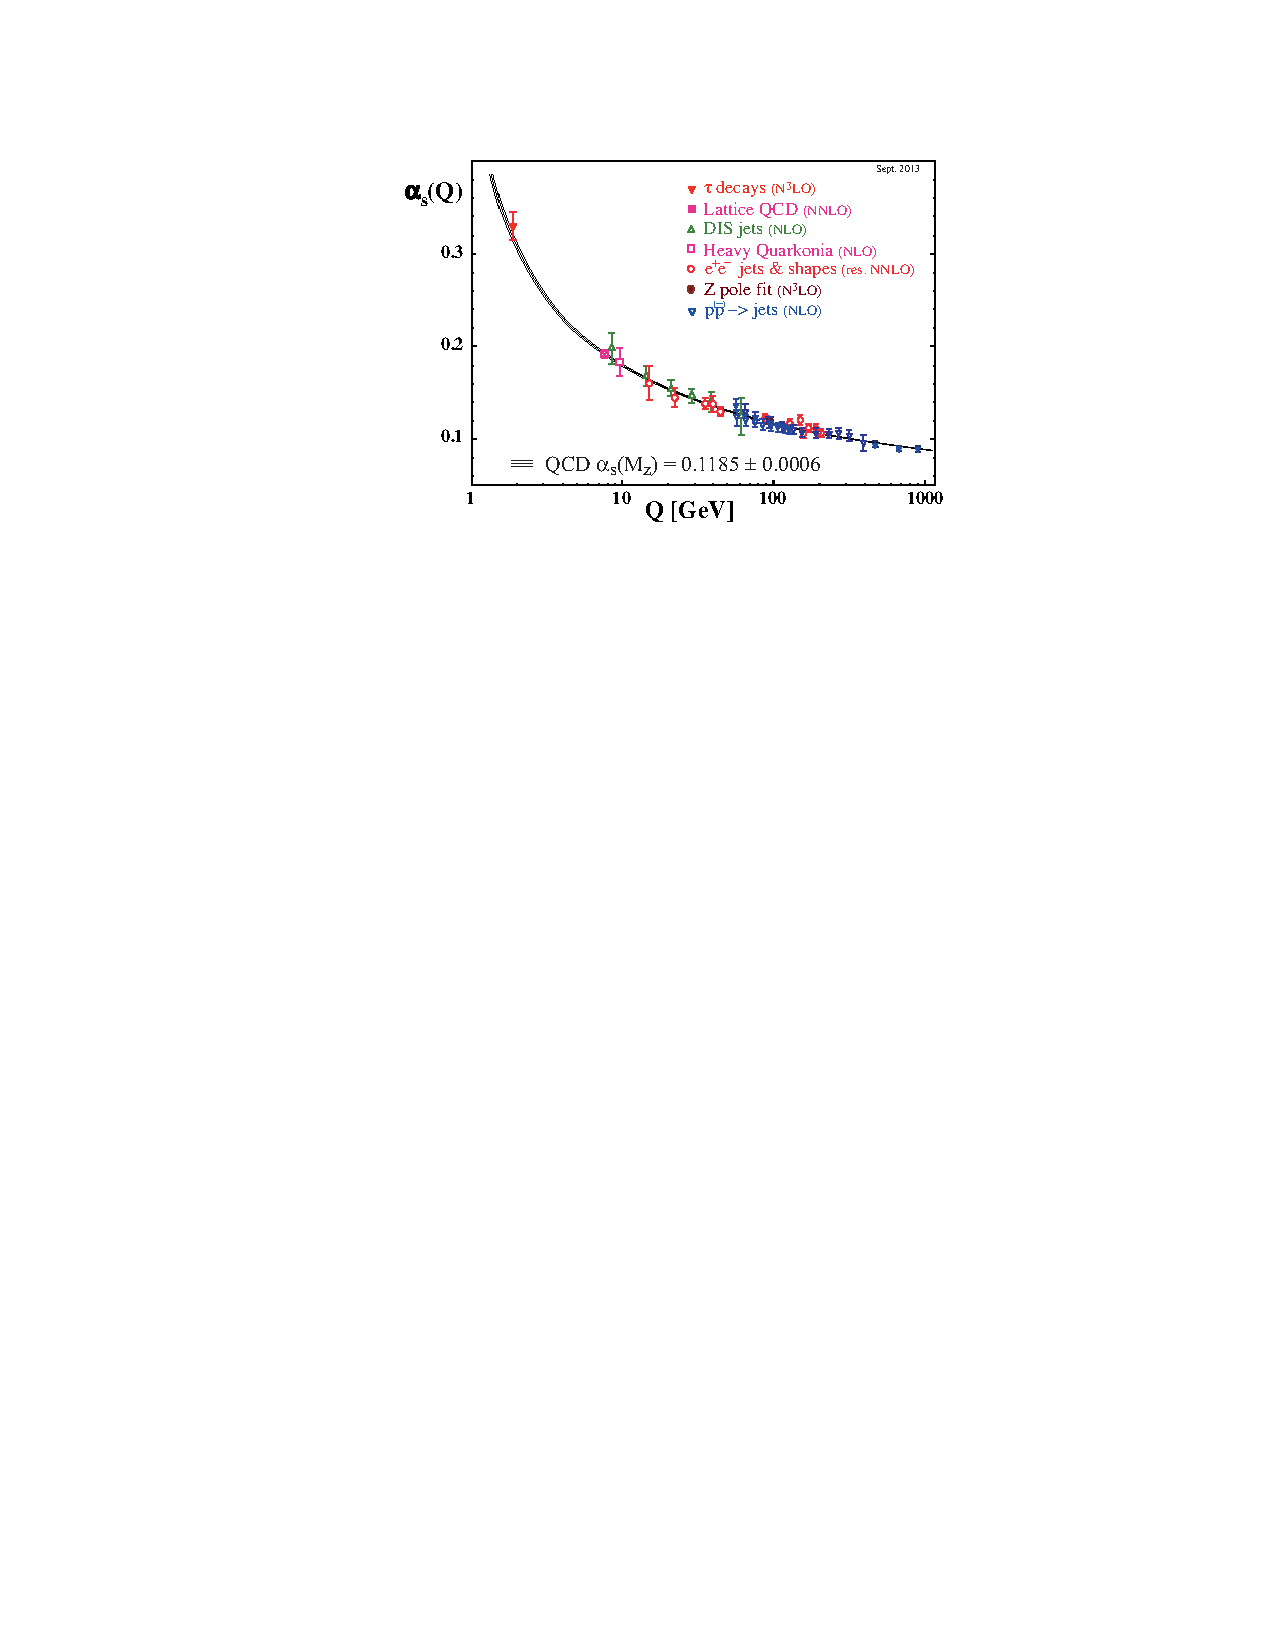
\includegraphics[width=0.80\textwidth]{figures/alphaS_running.pdf}
  \caption{The so-called ``running'' of $\alpha_S$ as the energy scale ~\cite{PhysRevD.98.030001}.} 
  \label{fig:alphaS}
\end{figure}

% Diagram
For experimental physics at the LHC, QCD is important even for studying electroweak processes.
Since we collide protons, the internal dynamics of the proton are an essential ingredient of Monte Carlo simulations.
The momentum fractions carried by the quarks and gluons are determined empirically, giving us the proton parton distribution functions.
Internal gluon loop corrections and the possibility of emitting extra gluons before or after the hard process can enhance the total cross section significantly for physics processes.
QCD activity resulting in charged hadrons may interfere with the ability to identify charged leptons in physics events of interest.
Lastly, the hadronic radiation from the interaction point irradiates the detector components. This changes their material properties over time.
\clearpage
\section{Proton parton distribution functions}

The quarks and gluons inside a proton are collectively called partons.
The parton distribution functions (PDFs) $f_i(x,Q^2)$ give the probability of finding inside the proton a quark or gluon with momentum fraction $x$, in a hard process with momentum transfer $Q$.
The PDF shapes are not calculated theoretically and are instead determined empirically by experimental data.

\begin{figure}[hb]
  \centering
    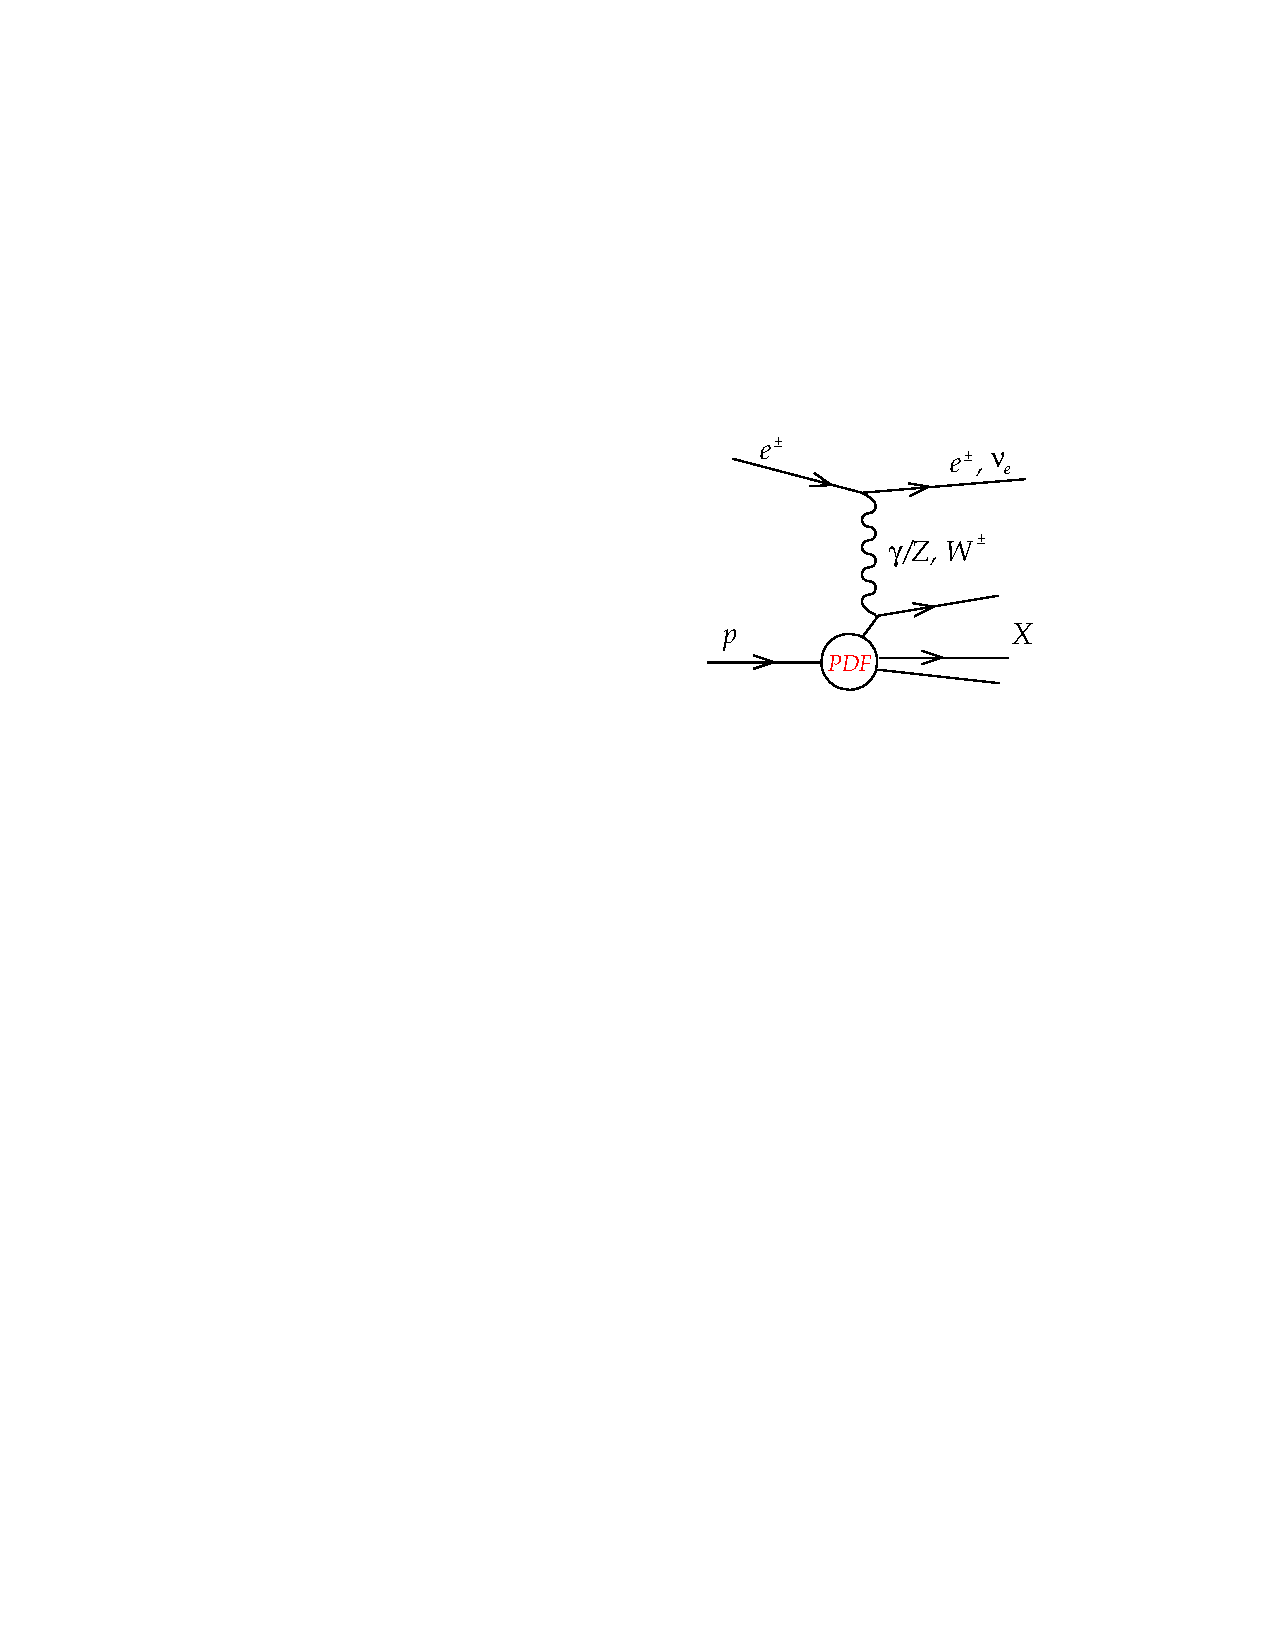
\includegraphics[width=0.50\textwidth]{figures/dis.pdf}
  \caption{Probing the PDFs with deep inelastic scattering. From \cite{Placakyte:2011az}.} 
  \label{fig:dis}
\end{figure}

The HERA experiment provided important data for the PDF determination by performing
deep inelastic scattering of electrons or positrons with protons, 
at center of mass energies of a few hundred \GeV.
Two different scattering processes can occur, the neutral current and charged current.
See Figure~\ref{fig:dis}.
In the charged current interaction, the cross sections of electron and positron on proton are sensitive to different quark PDFs.
%The neutral current $ep$ cross section can be expressed in terms of the structure functions $\tilde{F}$:
%\begin{equation}
%\frac{d^2 \sigma^{e^\pm p}_\mathrm{N.C.}}{dx\:dQ^2} = \frac{2 \pi \alpha^2}{xQ^4}\termLB Y_+ \tilde{F}^\pm_2 \mp Y_{-} x \tilde{F}^\pm_3 - y^2 \tilde{F}^\pm_L \termRB
%\end{equation}
%where $Y_\pm = 1 \pm (1-y^2)$ as a function of the inelasticity $y$.
%In general, $\tilde{F}_2$ dominates, $x\tilde{F^3}$ becomes important at higher $Q^2$,
%and $\tilde{F}_L$ only matters for significant $y$.
%The PDFs are directly related to these structure functions.
%Neglecting higher-order terms for the gluon density: $F_2$ is approximately the momentum sum of the 
%distributions of quarks and antiquarks ($F_2 \approx x\sum e_q^2 (q+\bar{q})$) 
%and $F_3$ is approximately their momentum difference ($xF_3 \approx x\sum 2e_qa_q(q-\bar{q}))$.
%
%The charged current $ep$ cross section can also be expressed in terms of structure functions.

In $p\bar{p}$ and $pp$ collisions at the Tevatron and LHC,
we can learn more about the proton PDFs through Standard Model precision measurements.
In particular, the Z boson differential cross section studied in this work contributes to the global fit of the quark distributions.
Meanwhile, ultraperipheral lead-lead heavy ion collisions are also an unconventional source of high energy photon probes which help us study the gluon distribution down to very small values of $x$ (see~\cite{Baltz:2007kq}).
Overall, the PDFs are an important quantity for simulating the Standard Model background in a search for new physics.
An example of the PDF set provided by the NNPDF collaboration at $Q=50 \GeV$ is shown in Figure~\ref{fig:pdfq50}.

\begin{figure}[hbtp]
  \centering
    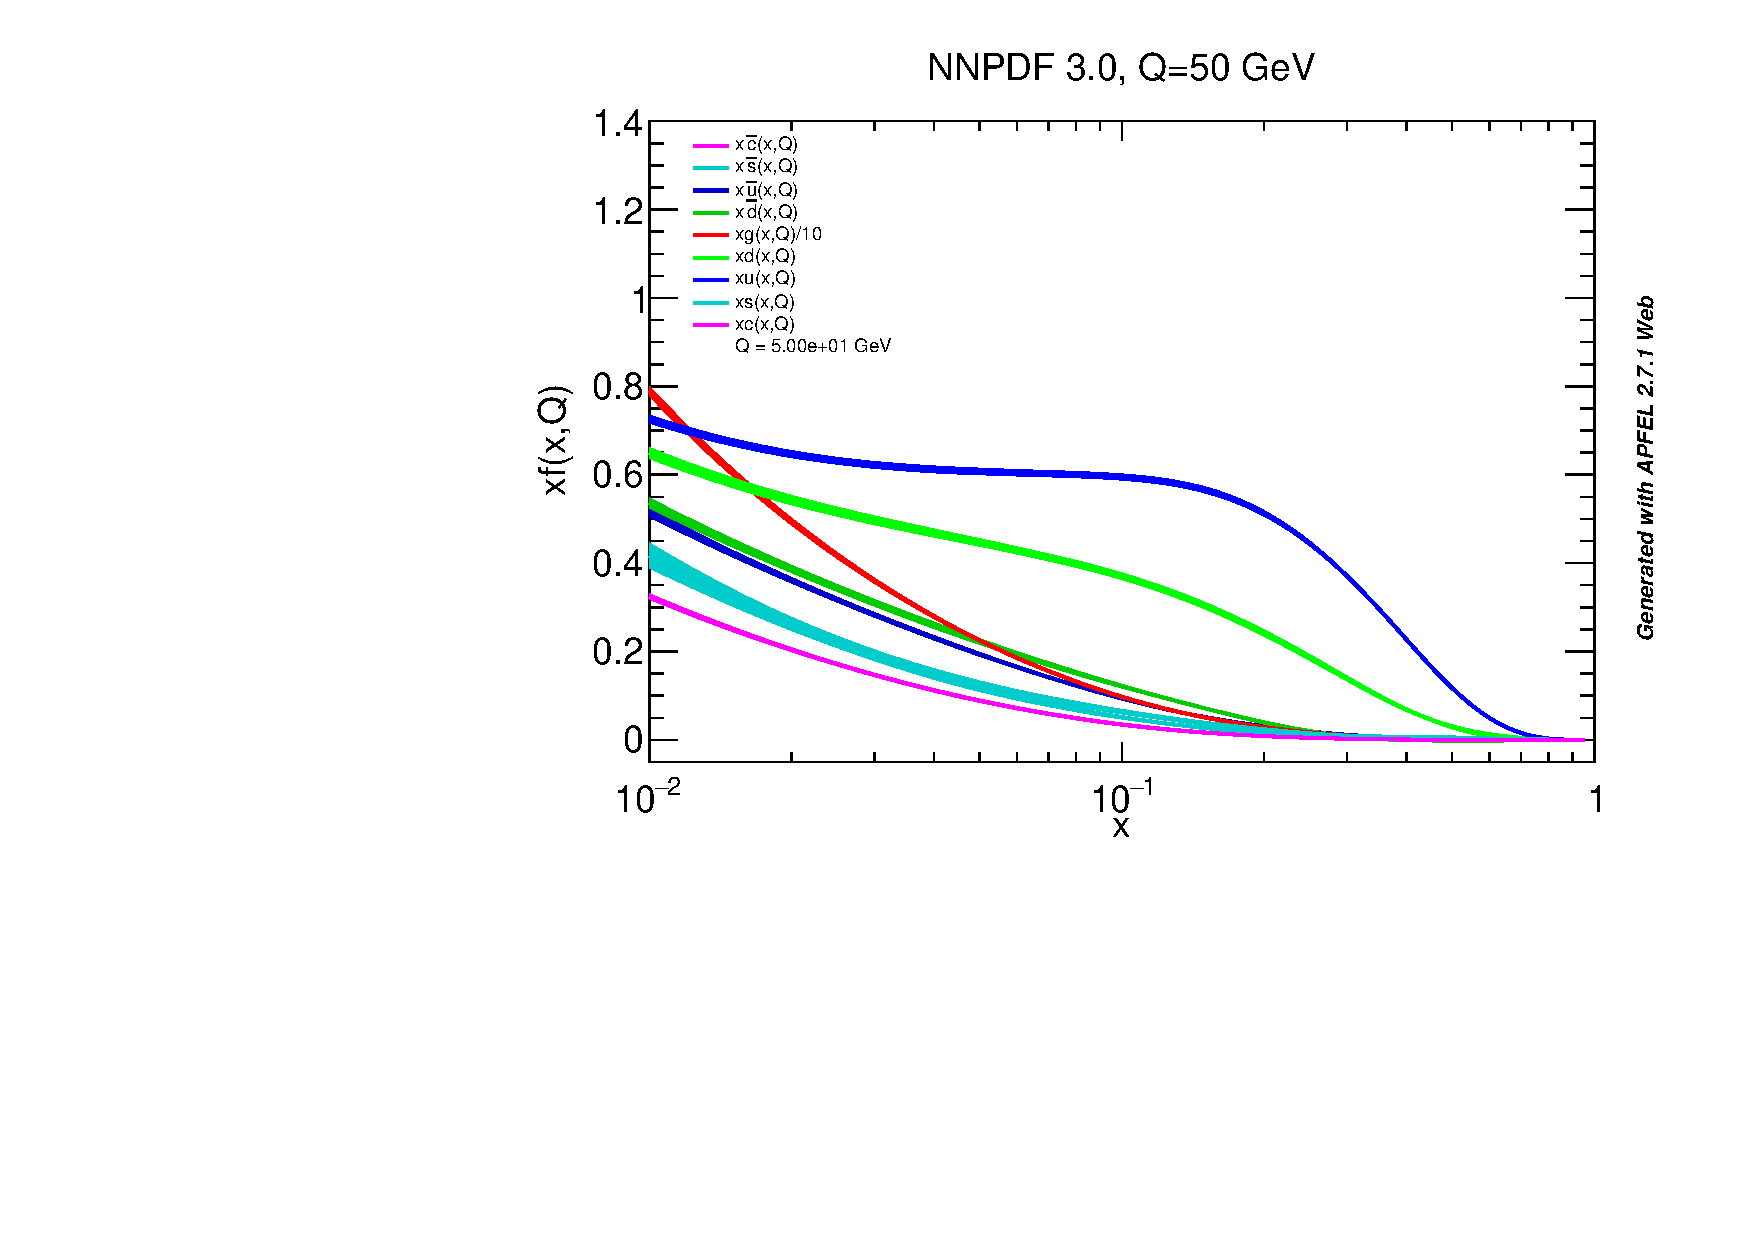
\includegraphics[width=0.90\textwidth]{figures/nnpdf30_115_Q50_v4.pdf}
  \caption{NNPDF 3.0 set at momentum transfer 50 \GeV. Presented in~\cite{nnpdf}.} 
  \label{fig:pdfq50}
\end{figure}

\section{New physics}
%In this work, we consider a scenario in which are produced a pair of charged leptons ($\ell^{+}\ell^{-}$, where $\ell=\Pe$ or $\Pgm$),
%consistent with the decay of a $\PZ$ boson, together with large missing transverse momentum ($\met$).

The study presented here considers one possible mechanism for producing weakly interacting massive particles at the LHC~\cite{Abercrombie:2015wmb}.
In this scenario, a $\PZ$ boson, produced in $pp$ collisions, recoils against a pair of DM particles, $\chi\overline\chi$.
The $\PZ$ boson subsequently decays into two charged leptons (electrons or muons), 
%producing a low-background dilepton signature, 
recoiling against $\met$ due to the undetected DM particles. 
We assume the final state dark matter particle $\chi$ is a Dirac fermion.

\begin{figure} % BSM models
 \centering
 \begin{tikzpicture} % ZH(inv)
  \begin{feynman}
   \vertex (q1) {\(\boldsymbol{\Pq}\)};
   \vertex [below= 3cm of q1] (q2) {\(\boldsymbol{\Paq}\)};
   \vertex [right= 1.6cm of q1] (a1);
   \vertex [below= 1.5cm of a1] (a2);
   \vertex [right= 1.6cm of a2] (b1);
   \vertex [right= 1.6cm of b1] (c1);
   \vertex [above= 1.3cm of c1] (c2);
   \vertex [below= 1.3cm of c1] (c3);
   \vertex [right= 1cm of c2] (d1);
   \vertex [right= 1cm of c3] (d2);
   \vertex [above= 0.3cm of d1] (f1) {\(\boldsymbol{\ell}\)};
   \vertex [below= 0.3cm of d1] (f2) {\(\boldsymbol{\bar{\ell}}\)};
   \vertex [above= 0.3cm of d2] (f3) {\(\boldsymbol{\chi}\)};
   \vertex [below= 0.3cm of d2] (f4) {\(\boldsymbol{\bar{\chi}}\)};
   
   \diagram* {
    (q1) -- [fermion, very thick] (a2),
    (q2) -- [anti fermion, very thick] (a2),
    (a2) -- [boson, very thick, edge label'=\(\boldsymbol{\Z^*}\)] (b1),
    (b1) -- [boson, very thick, edge label=\(\boldsymbol{\Z}\)] (c2),
    (b1) -- [scalar, very thick, edge label=\(\boldsymbol{\Hi}\)] (c3),
    (c2) -- [fermion, very thick] (f1),
    (c2) -- [anti fermion, very thick] (f2),
    (c3) -- [fermion, very thick] (f3),
    (c3) -- [anti fermion, very thick] (f4),
   };
  \end{feynman}
 \end{tikzpicture} \hspace{1cm}
 \begin{tikzpicture} % Simplified model spin-0 mediator
  \begin{feynman}
   \vertex (g1) {\(\boldsymbol{}\)};
   \vertex [below= 3.6cm of g1] (g2) {\(\boldsymbol{}\)};
   \vertex [right= 1.4cm of g1] (a1);
   \vertex [right= 1.4cm of g2] (a2);
   \vertex [below= 0.8cm of a1] (a3);
   \vertex [above= 0.8cm of a2] (a4);
   \vertex [right= 1.4cm of a3] (b1);
   \vertex [right= 1.4cm of a4] (b2);
   \vertex [right= 1.4cm of b1] (c1);
   \vertex [right= 1.4cm of b2] (c2);
   \vertex [right= 1cm of c1] (d1);
   \vertex [right= 1cm of c2] (d2);
   \vertex [above= 0.3cm of d1] (f1) {\(\boldsymbol{\ell}\)};
   \vertex [below= 0.3cm of d1] (f2) {\(\boldsymbol{\bar{\ell}}\)};
   \vertex [above= 0.3cm of d2] (f3) {\(\boldsymbol{\chi}\)};
   \vertex [below= 0.3cm of d2] (f4) {\(\boldsymbol{\bar{\chi}}\)};
   \vertex [below = 0.2cm of b2] (dm1) {\(\boldsymbol{g_\Pq}\)};
   \vertex [below = 0.2cm of c2] (dm2) {\(\boldsymbol{g_\mathrm{DM}}\)};
   
   \diagram* {
    (g1) -- [gluon, very thick] (a3),
    (g2) -- [gluon, very thick] (a4),
    (a3) -- [fermion, very thick, edge label'=\(\boldsymbol{\bar{\Top}}\)] (a4) -- [fermion, very thick, edge label=\(\boldsymbol{\Top}\)] (b2) -- [fermion, very thick, edge label=\(\boldsymbol{\bar{\Top}}\)] (b1) -- [fermion, very thick, edge label'=\(\boldsymbol{\Top}\)] (a3),
    (b1) -- [boson, very thick, edge label=\(\boldsymbol{\Z}\)] (c1),
    (b2) -- [scalar, very thick, edge label=\(\boldsymbol{\phi}\)] (c2),
    (c1) -- [fermion, very thick] (f1),
    (c1) -- [anti fermion, very thick] (f2),
    (c2) -- [fermion, very thick] (f3),
    (c2) -- [anti fermion, very thick] (f4),
   };
  \draw[fill=blue,line width=0pt] (b2) circle(1.5mm);
  \draw[fill=violet,line width=0pt] (c2) circle(1.5mm);
  \end{feynman}
 \end{tikzpicture} \vspace{1cm}
 
 \begin{tikzpicture} % Simplified model spin-1 mediator
  \begin{feynman}
   \vertex (q1) {\(\boldsymbol{\Pq}\)};
   \vertex [below= 3.6cm of q1] (q2) {\(\boldsymbol{\Paq}\)};
   \vertex [right= 2cm of q1] (a1);
   \vertex [right= 2cm of q2] (a2);
   \vertex [below= 0.8cm of a1] (a3);
   \vertex [above= 0.8cm of a2] (a4);
   \vertex [right= 2cm of a3] (b1);
   \vertex [right= 2cm of a4] (b2);
   \vertex [right= 1.5cm of b1] (c1);
   \vertex [right= 1.5cm of b2] (c2);
   \vertex [above= 0.3cm of c1] (f1) {\(\boldsymbol{\ell}\)};
   \vertex [below= 0.3cm of c1] (f2) {\(\boldsymbol{\bar{\ell}}\)};
   \vertex [below= 0.2cm of c2] (U) {\(\boldsymbol{\mathcal{U}/\mathcal{G}}\)};
   
   \diagram* {
    (q1) -- [fermion, very thick] (a3),
    (a3) -- [fermion, very thick] (a4),
    (q2) -- [anti fermion, very thick] (a4),
    (a3) -- [boson, very thick, edge label=\(\boldsymbol{\Z}\)] (b1),
    (a4) -- [ghost, very thick] (U),
    (b1) -- [fermion, very thick] (f1),
    (b1) -- [anti fermion, very thick] (f2),
   };
  \draw[fill=black,line width=0pt] (a4) circle(2.2mm);
  \draw[pattern=north east lines, pattern color=white] (a4) circle(2.2mm);
  \end{feynman}
 \end{tikzpicture} \hspace{1cm}  
 \begin{tikzpicture} % ADD/unparticles
  \begin{feynman}
   \vertex (q1) {\(\boldsymbol{\Pq}\)};
   \vertex [below= 3.6cm of q1] (q2) {\(\boldsymbol{\Paq}\)};
   \vertex [right= 2cm of q1] (a1);
   \vertex [right= 2cm of q2] (a2);
   \vertex [below= 0.8cm of a1] (a3);
   \vertex [above= 0.8cm of a2] (a4);
   \vertex [right= 2cm of a3] (b1);
   \vertex [right= 2cm of a4] (b2);
   \vertex [right= 1.5cm of b1] (c1);
   \vertex [right= 1.5cm of b2] (c2);
   \vertex [above= 0.3cm of c1] (f1) {\(\boldsymbol{\ell}\)};
   \vertex [below= 0.3cm of c1] (f2) {\(\boldsymbol{\bar{\ell}}\)};
   \vertex [above= 0.3cm of c2] (f3) {\(\boldsymbol{\chi}\)};
   \vertex [below= 0.3cm of c2] (f4) {\(\boldsymbol{\bar{\chi}}\)};
   \vertex [below = 0.2cm of a4] (dm1) {\(\boldsymbol{g_\Pq}\)};
   \vertex [below = 0.2cm of b2] (dm2) {\(\boldsymbol{g_\mathrm{DM}}\)};
   
   \diagram* {
    (q1) -- [fermion, very thick] (a3),
    (a3) -- [fermion, very thick] (a4),
    (q2) -- [anti fermion, very thick] (a4),
    (a3) -- [boson, very thick, edge label=\(\boldsymbol{\Z}\)] (b1),
    (a4) -- [boson, very thick, edge label=\(\boldsymbol{\mathcal{A}}\)] (b2),
    (b1) -- [fermion, very thick] (f1),
    (b1) -- [anti fermion, very thick] (f2),
    (b2) -- [fermion, very thick] (f3),
    (b2) -- [anti fermion, very thick] (f4),
   };
  \draw[fill=blue,line width=0pt] (a4) circle(1.5mm);
  \draw[fill=violet,line width=0pt] (b2) circle(1.5mm);
  \end{feynman}
 \end{tikzpicture}
 \caption{Some diagrams beyond the Standard Model in which are produced two charged leptons and missing energy. Clockwise from upper left: associated production of an invisible Higgs boson; gluon-induced production of a Z boson and a massive spin-0 dark matter mediator via top-quark loop; production of a Z boson and a massive spin-1 dark matter mediator; production of a Z boson in association with gravitons (ADD model) or unparticles.} \label{fig:BSMdiagrams}
\end{figure}

\subsection{Simplified models}
Four simplified models of DM production via an $s$-channel mediator exchange are considered.
In these models, the mediator has a spin of 1 (0) and vector or axial-vector (scalar or pseudoscalar) couplings to quarks and DM particles.
The free parameters of each model are the masses $m_{\rm med}$ and $m_{\rm DM}$ of the mediator and DM particle, respectively, as well as the coupling
constant $g_{\Pq}$ ($g_{\rm DM}$) between the mediator and the quarks (DM particles).
The vector coupling model can be described with the following Lagrangian:

\begin{equation*}
\mathcal{L}_{\text{vector}} = g_{\rm DM} {Z'}_{\mu}\overline{\chi}\gamma^{\mu}\chi  + g_{\Pq} \sum_{\Pq} {Z'}_{\mu} \overline{\Pq}\gamma^{\mu}\Pq,
\end{equation*}

\noindent where the spin-1 mediator is denoted as $\PZ'$ and the SM quark fields are referred to as \PQq and $\overline{\PQq}$.
The Lagrangian for an axial-vector coupling is obtained by making the replacement $\gamma^\mu\rightarrow\gamma^5\gamma^\mu$.
In the case of a spin-0 mediator $\phi$, the couplings between mediator and quarks are assumed to be Yukawa-like, with $g_{\Pq}$ acting as a 
multiplicative modifier for the SM Yukawa coupling ${y_{\Pq} = \sqrt{2}m_{\Pq}/v}$ (where $v = 246 \GeV$ is the SM Higgs field vacuum expectation value),
leading to the Lagrangian:

\begin{equation*}
\mathcal{L}_{\text{scalar}} = g_{\rm DM} {\phi}\overline{\chi}\chi  + g_{\Pq} \frac{\phi}{\sqrt{2}}\sum_{\Pq} y_{\Pq} \overline{\Pq}\Pq.
\end{equation*}

\noindent The Lagrangian with pseudoscalar couplings is obtained by inserting a factor of $i\gamma^5$ into each of the two terms (i.e., $\bar\chi\chi \to i\bar\chi\gamma^5\chi$ and $\bar \Pq \Pq \to i\bar \Pq\gamma^5 \Pq$). Example diagrams of DM production via spin-0 and spin-1 mediators are shown in Fig.~\ref{fig:BSMdiagrams} (upper right and lower right, respectively).

%\begin{figure}[!hbtp]
%  \centering
%    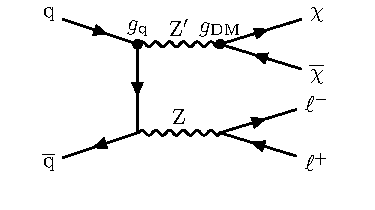
\includegraphics[width=0.45\textwidth]{figures/dmSimpFeynman.pdf}
%    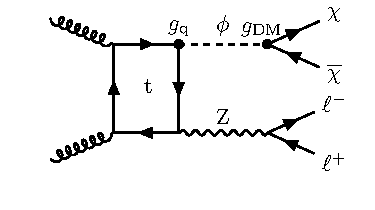
\includegraphics[width=0.45\textwidth]{figures/dmSimpFeynman_spin0.pdf}
%    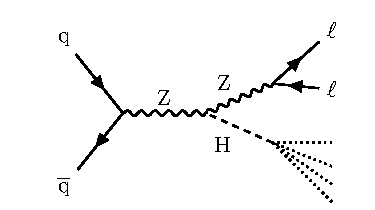
\includegraphics[width=0.45\textwidth]{figures/higgsInvisibleFeynman.pdf}
%    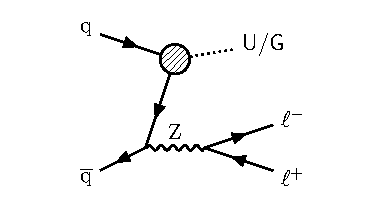
\includegraphics[width=0.45\textwidth]{figures/graph_UG.pdf}
%  \caption{Feynman diagrams illustrative of the processes beyond the SM considered in this paper:
%    (upper left)~DM production in a simplified model with a spin-1 mediator $\PZ'$;
%    (upper right)~DM production in a simplified model with a spin-0 mediator $\phi$;
%    (lower left)~production of a Higgs boson in association with Z boson with subsequent decay of the Higgs boson into invisible particles;
%    (lower right)~unparticle or graviton production. The diagrams were drawn using the {\sc TikZ-Feynman} package~\cite{Ellis:2016jkw}.
%  } 
%      \label{fig:Feynman}
%\end{figure}

\subsection{Invisible Higgs bosons}

A primary focus of the LHC physics program after the discovery of the Higgs boson ~\cite{AtlasPaperCombination,CMSPaperCombination} by
the ATLAS and CMS Collaborations is the study of the properties of this new particle. The observation of a sizable branching
fraction of the Higgs boson to invisible states~\cite{Ghosh:2012ep,Martin:1999qf,Bai:2011wz} would be a strong sign
of BSM physics.  Supersymmetric (SUSY) models embodying R-parity conservation contain a stable neutral lightest SUSY
particle (LSP), e.g., the lightest neutralino~\cite{Belanger:2001am}, leading to the possibility of decays of the Higgs boson into pairs of LSPs.
Certain models with extra spatial dimensions predict graviscalars that could mix with the
Higgs boson~\cite{Giudice:2000av}.  As a consequence, the Higgs boson could oscillate
to a graviscalar and disappear from the SM brane. The signature would be
equivalent to an invisible decay of the Higgs boson. There could also be contributions
from Higgs boson decays into graviscalars~\cite{Battaglia:2004js}.
Other ``Higgs portal'' models~\cite{Baek:2012se,Djouadi:2011aa,Djouadi:2012zc} construct
a generic connection between SM and DM particles via a Higgs boson mediator.
This work considers decays into invisible particles of an SM-like Higgs boson produced in association with a $\PZ$ boson, as shown in Fig.~\ref{fig:BSMdiagrams} (upper left).

\subsection{Extra dimensions}

A popular BSM paradigm considered here is the Arkani-Hamed--Dimopoulos--Dvali (ADD) model with large extra spatial dimensions~\cite{arkani98:hlz,arkani99:hlz,han99:hlz}, which
is motivated by the hierarchy problem, i.e., the disparity between the electroweak unification
scale ($M_\mathrm{EW} \sim 1\TeV$) and the Planck scale ($M_\mathrm{Pl} \sim 10^{16}\TeV$).
This model predicts graviton (\cPG) production via the process $\PQq\PAQq \rightarrow \PZ + \cPG$. The graviton escapes
detection, leading to a mono-$\PZ$ signature (Fig.~\ref{fig:BSMdiagrams}, lower right).
In the ADD model, the apparent Planck scale in four space-time dimensions
is given by $M_\mathrm{Pl}^2 \approx M_\mathrm{D}^{n+2}R^n$, where $M_\mathrm{D}$ is the true Planck scale of
the full $n$+4 dimensional space-time and $R$ is the compactification radius of the extra
dimensions. Assuming $M_\mathrm{D}$ is of the same order as $M_\mathrm{EW}$, the observed large value
of $M_\mathrm{Pl}$ points to an $R$ of order 1 mm to 1 fm for 2 to 7 extra dimensions. The consequence of
the large compactification scale is that the mass spectrum of the Kaluza--Klein graviton states
becomes nearly continuous, resulting in a broad $\PZ$ boson transverse momentum (\PT) spectrum.

\subsection{Unparticles}

The final BSM model considered in this work is the phenomenologically interesting concept of unparticles, which appear in the low-energy limit of conformal field theories.
In the high-energy regime, a new, scale invariant Banks--Zaks field with a nontrivial infrared fixed point is introduced~\cite{Banks:1981nn}.
The interaction between the SM and Banks--Zaks sectors is mediated by particles of large mass scale $M_{\textsf{U}}$, below which the interaction is suppressed and can be treated
via an effective field theory (EFT). The low-energy regime will include unparticles, which have phase space factors equivalent to those of a noninteger
number of ordinary particles~\cite{Kang:2014cia,Rinaldi:2014gha,Cheng:1988zx}. 
In this work, the emission of spin-0 unparticles from SM quarks is considered.
Because of the weakness of the unparticle interactions with the SM fields, the unparticle evades detection.
The EFT Lagrangian used to interpret the results is defined as follows:

\begin{equation*}
\mathcal{L}_{U}  = \frac{\lambda}{\LU^{\dU-1}} \mathcal{O}_{\textsf{U}} \overline{\PQq}\PQq,
\end{equation*}

\noindent where $\lambda$ represents the coupling between the SM and unparticle fields, \LU is the cutoff scale of the EFT, and \dU is the characteristic scaling dimension of the theory.
The unparticle operator is denoted as $\mathcal{O}_{\textsf{U}}$.
A representative Feynman diagram of the interaction is shown in Fig.~\ref{fig:BSMdiagrams} (lower right).


